\section{Electrostatic transduction and sensitivity}

\subsection*{Q6: Static phase shift versus DC voltage}

Considering only the perpendicular field component, the comb-drive
capacitance varies linearly with the engagement length $d_{0}+\xm$:
\begin{equation}
  C(\xm) = N\,\varepsilon_{0}\,\frac{t\,(d_{0}+\xm)}{h},
  \qquad
  \frac{dC}{d\xm} = \frac{N\,\varepsilon_{0}\,t}{h}
                  = \SI{7.08e-11}{\farad\per\meter}.
\end{equation}
The electrostatic force on the mass therefore depends only on voltage:
\begin{equation}
  \Fe = \tfrac{1}{2}\,\Vd^{2}\,\frac{dC}{d\xm}
      = \tfrac{1}{2}\,\Vd^{2}\,\frac{N\,\varepsilon_{0}\,t}{h}.
  \label{eq:Fcomb}
\end{equation}
Static balance with the spring force ($\Fe=k\xm$) yields the displacement
\begin{equation}
  \xm(\Vd) \;=\; \frac{\Vd^{2}\,N\,\varepsilon_{0}\,t}{2 k h},
  \qquad
  g(\Vd) \;=\; g_{0} + \xm(\Vd).
  \label{eq:gV}
\end{equation}
Substituting into Eq.~\ref{eq:phase} gives the phase shift plotted in
Fig.~\ref{fig:q6}. It is symmetric in $\Vd$ and quadratic. At
$\Vd=\pm 50\,\mathrm{V}$ the gap only changes by $\xm\approx \SI{2.2}{\nano\meter}$
(1\% of $g_{0}$), so $|\Delta\phi|$ stays around $\SI{50}{\milli\radian}$. Reaching
$\pi$ radians of phase shift would need a much higher bias.

\begin{figure}[H]
\centering
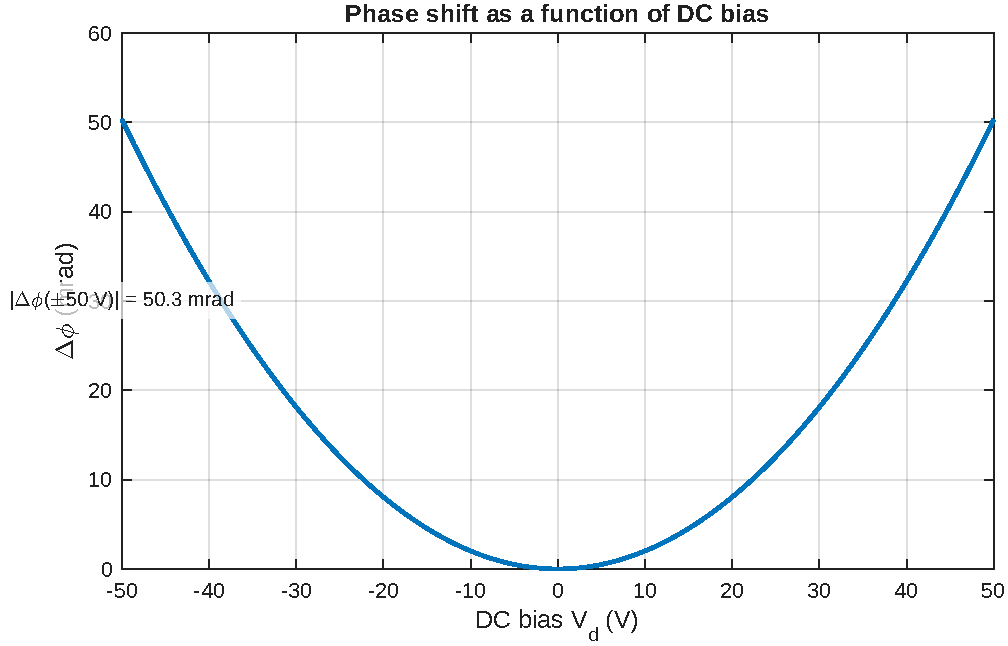
\includegraphics[width=0.78\textwidth]{figures/q6_phase_vs_V.pdf}
\caption{Static phase shift $\Delta\phi$ as a function of the DC bias
$\Vd\in[-50,\,+50]\,\mathrm{V}$. The shift is symmetric and quadratic in
$\Vd$, in line with Eq.~\ref{eq:Fcomb}.}
\label{fig:q6}
\end{figure}

\subsection*{Q7: Pull-in instability of the comb drive}

\paragraph{Case A, perpendicular field only.}
The overlap force in Eq.~\ref{eq:Fcomb} does not depend on $\xm$, so
$dF_{e}/d\xm = 0 < k$ for any $\Vd$. The single equilibrium
$\xm = \tfrac{1}{2}\Vd^{2}(dC/d\xm)/k$ is always stable. \emph{No pull-in.}
This is why comb drives are preferred over parallel-plate actuators when long
strokes are needed.

\paragraph{Case B, including finger-tip parallel-plate capacitance.}
When the mass moves into the comb, the gap between each finger tip and the
opposing anchor shrinks from $g_{t,0}=L_{c}-d_{0}=\SI{1}{\micro\meter}$ to
$g_{t}=g_{t,0}-\xm$. The additional capacitance and force per finger pair are
\begin{equation}
  C_{\mathrm{tip}}(\xm) = N\,\varepsilon_{0}\,\frac{W_{c}\,t}{g_{t,0}-\xm},
  \quad
  F_{\mathrm{tip}}(\xm) = \tfrac{1}{2}\,\Vd^{2}\,
                          \frac{N\,\varepsilon_{0}\,W_{c}\,t}{(g_{t,0}-\xm)^{2}}.
\end{equation}
Total force balance:
\begin{equation}
  k\xm = \tfrac{1}{2}\Vd^{2}\Biggl[\,
         \frac{N\varepsilon_{0}t}{h}
         + \frac{N\varepsilon_{0}W_{c}t}{(g_{t,0}-\xm)^{2}}\,\Biggr].
\end{equation}
Pull-in occurs when the small-signal stability condition $dF/d\xm = k$ is
reached:
\begin{equation}
  \Vd^{2}\,\frac{N\,\varepsilon_{0}\,W_{c}\,t}{(g_{t,0}-\xm)^{3}} = k.
\end{equation}
Eliminating $\Vd^{2}$ between the two equations gives an implicit relation
for the pull-in gap $u\equiv g_{t,0}-x_{\mathrm{pi}}$:
\begin{equation}
  g_{t,0} \;=\; \frac{3u}{2} + \frac{u^{3}}{2 h W_{c}}.
\end{equation}
Numerically, $u\approx\SI{0.60}{\micro\meter}$ (so
$x_{\mathrm{pi}}\approx\SI{0.40}{\micro\meter}$), giving the pull-in voltage
\begin{equation}
  V_{\mathrm{PI}} \;=\; \sqrt{\frac{k\,u^{3}}{N\,\varepsilon_{0}\,W_{c}\,t}}
                  \;\approx\; \SI{347}{\volt}.
\end{equation}
The mass-to-waveguide contact would only happen at
$\Vd \approx \sqrt{2 k g_{0}/(dC/d\xm)} \approx \SI{477}{\volt}$, so finger-tip
pull-in is what limits operation. As long as the bias stays well below
$\sim\!\SI{350}{\volt}$, Case A is a good model and the device behaves linearly.
